%!TEX root = ../../super_main.tex

\section{Vision Representation}
\label{sec:vision_representation}

With the two orientation question, and hereby the four quadrants, decided upon, we have tried to to make two vision representations, namely the metaphor- and the proposition representation.

\subsection{Metaphor Representation}
\label{sub:metaphor_representation}

\begin{figure}[!htbp]
	\centering
	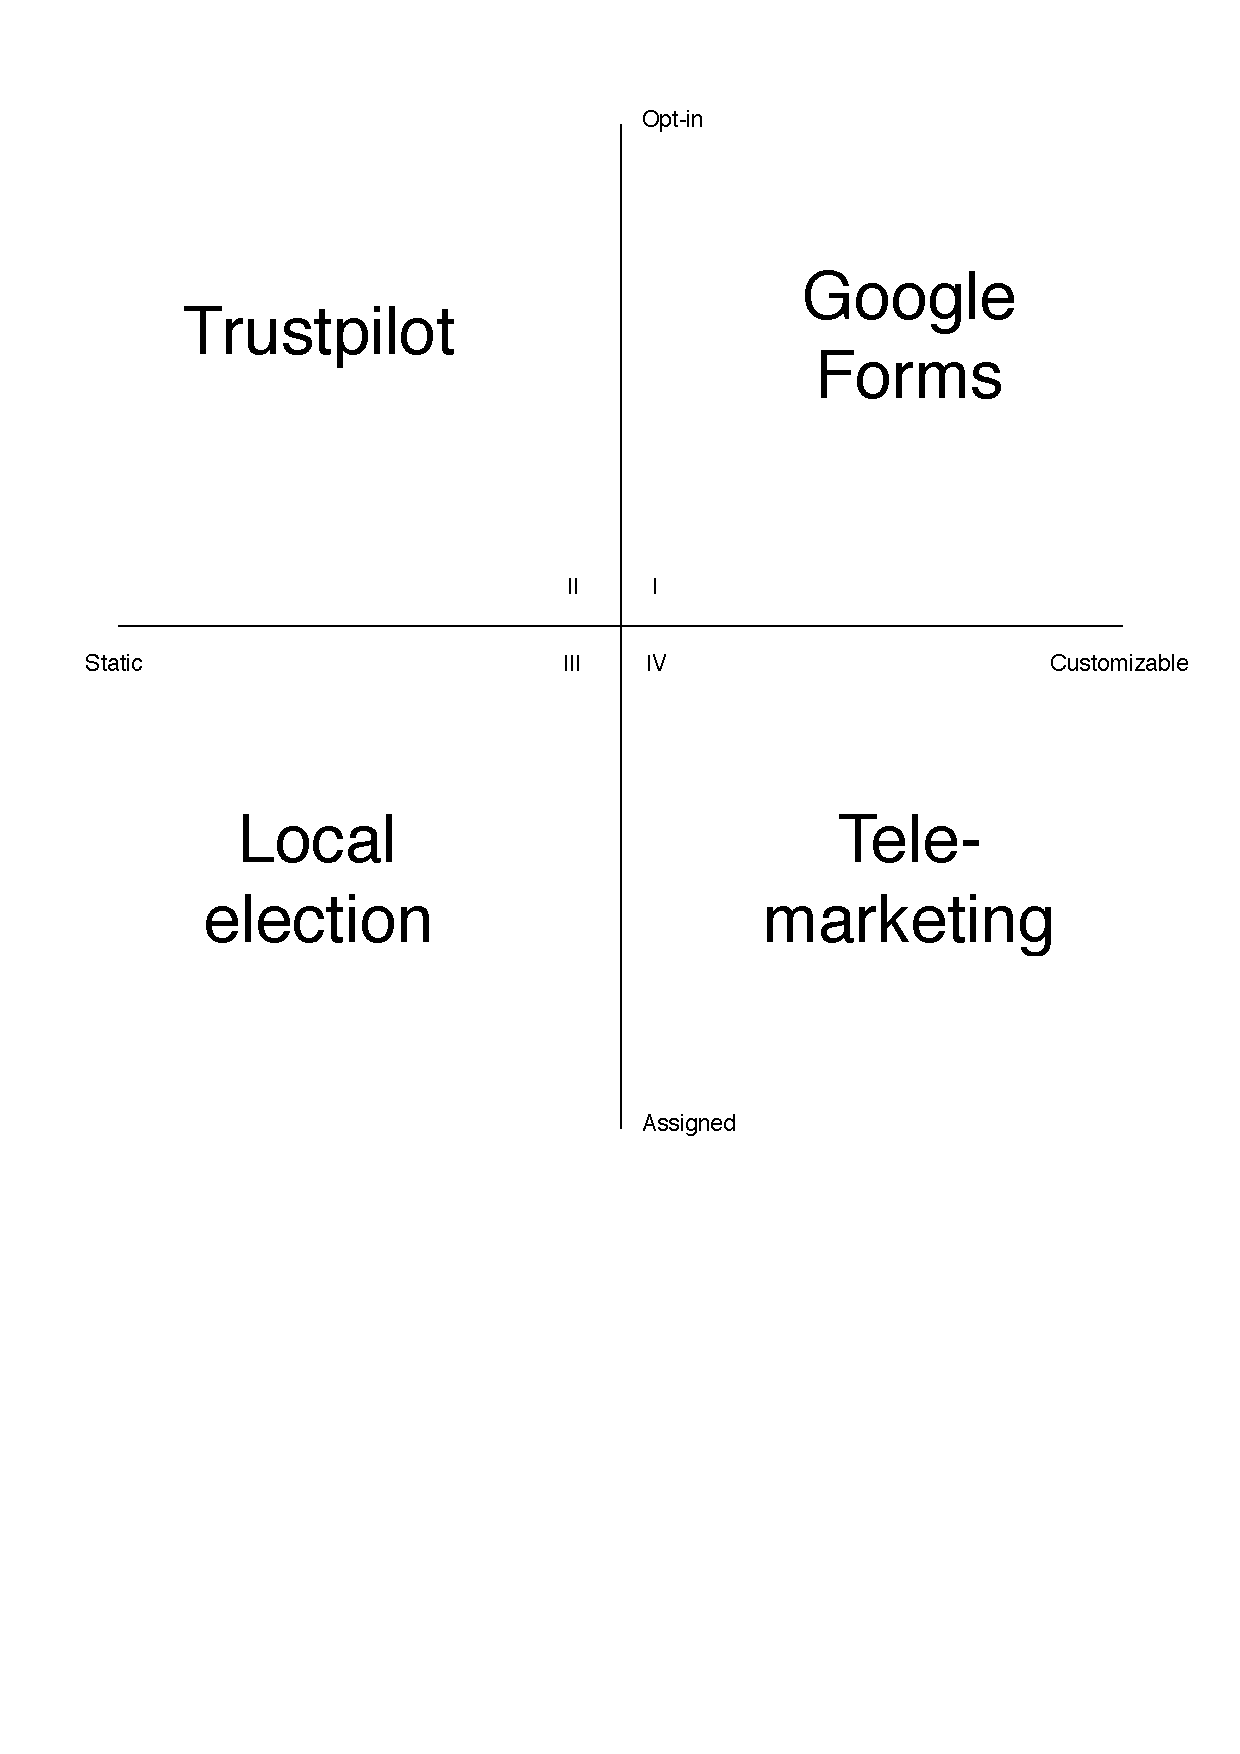
\includegraphics[width=0.8\textwidth]{graphic/problem_analysis/vision/metaphor.pdf}
	\caption{Four metaphors based upon the four quadrants.}
	\label{fig:metaphor}
\end{figure}
\FloatBarrier

\subsection{Proposition Representation}

\begin{figure}[!htbp]
	\centering
	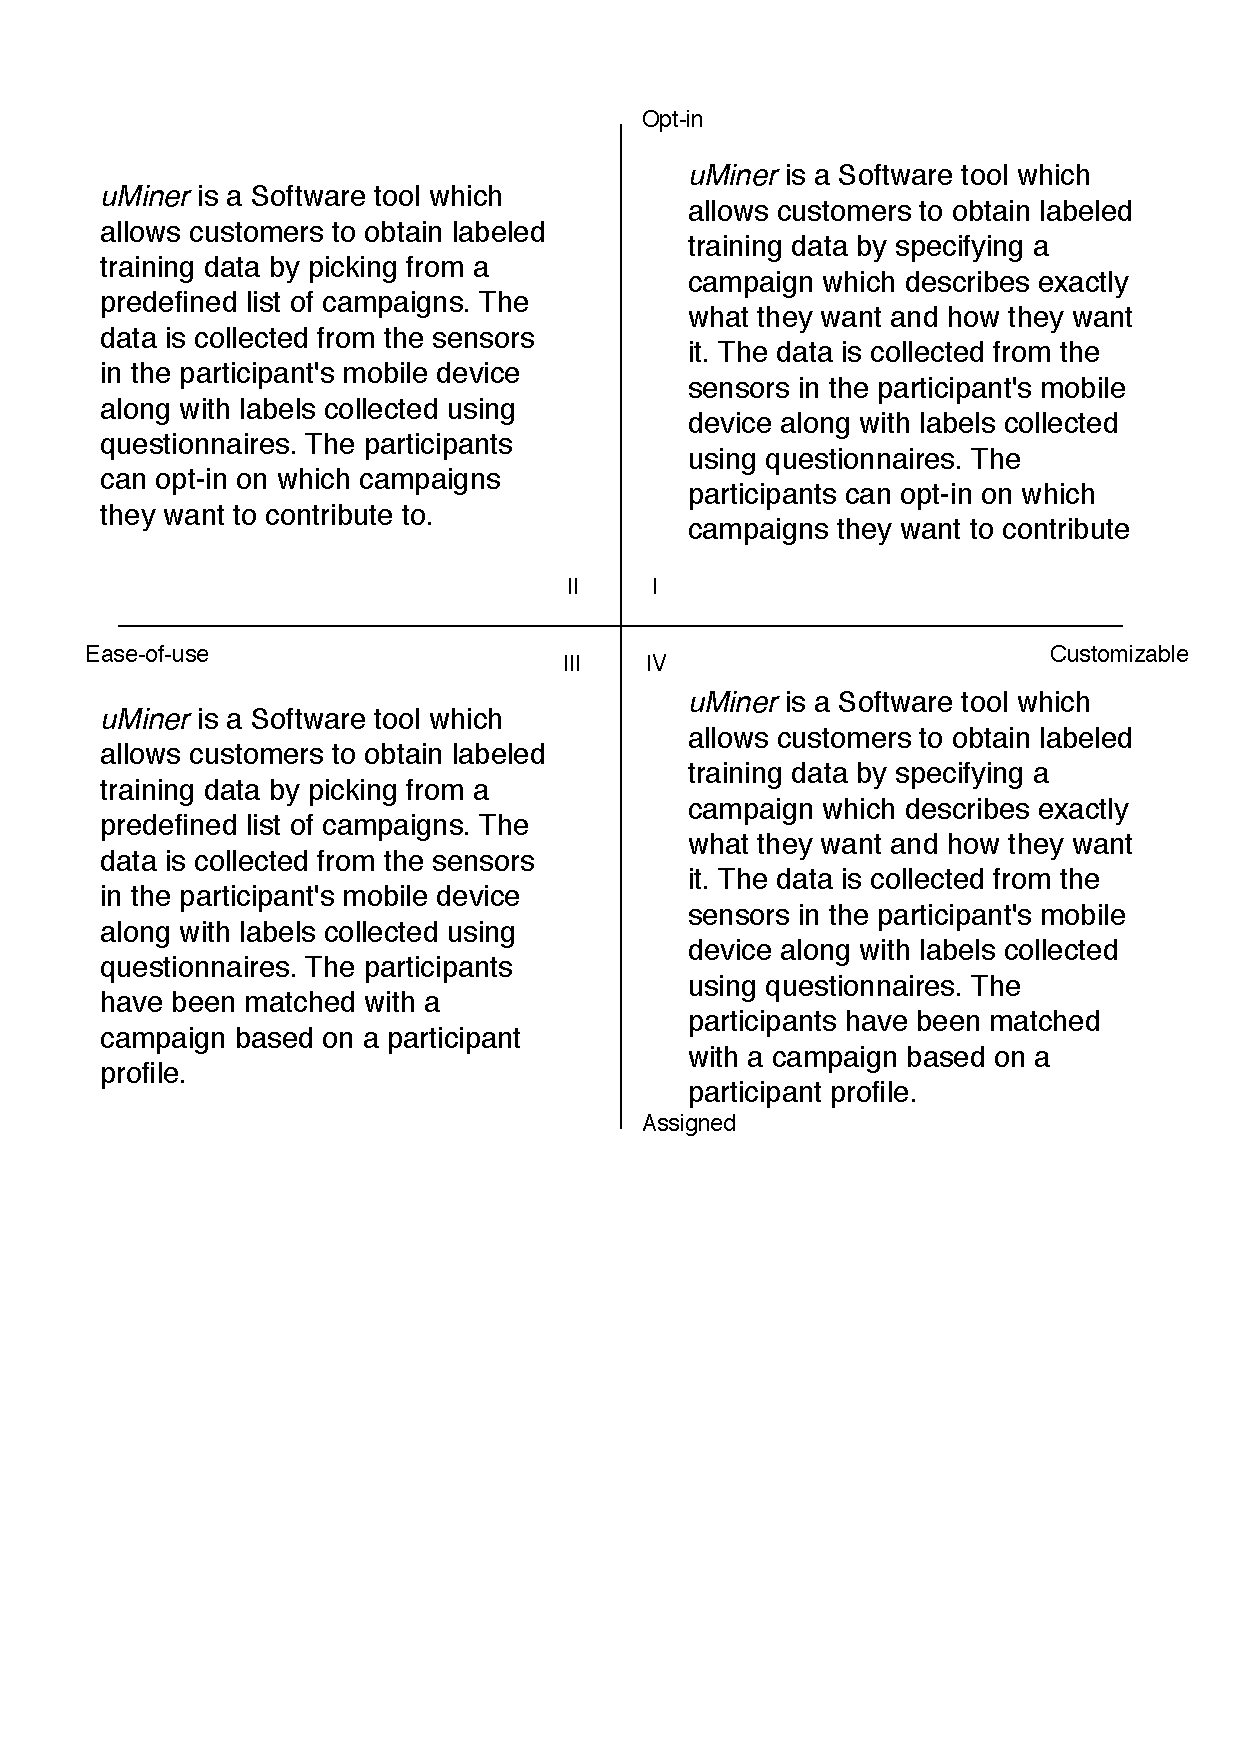
\includegraphics[width=0.8\textwidth]{graphic/problem_analysis/vision/propositions.pdf}
	\caption{Four propositions based upon the opposing questions.}
	\label{fig:proposition}
\end{figure}
\FloatBarrier

\todo[inline]{Figuren (\figref{fig:system_vision}) skal vist ikke lige stå her, måske i sektionen nedenunder}
\begin{figure}[!htbp]
    \centering
    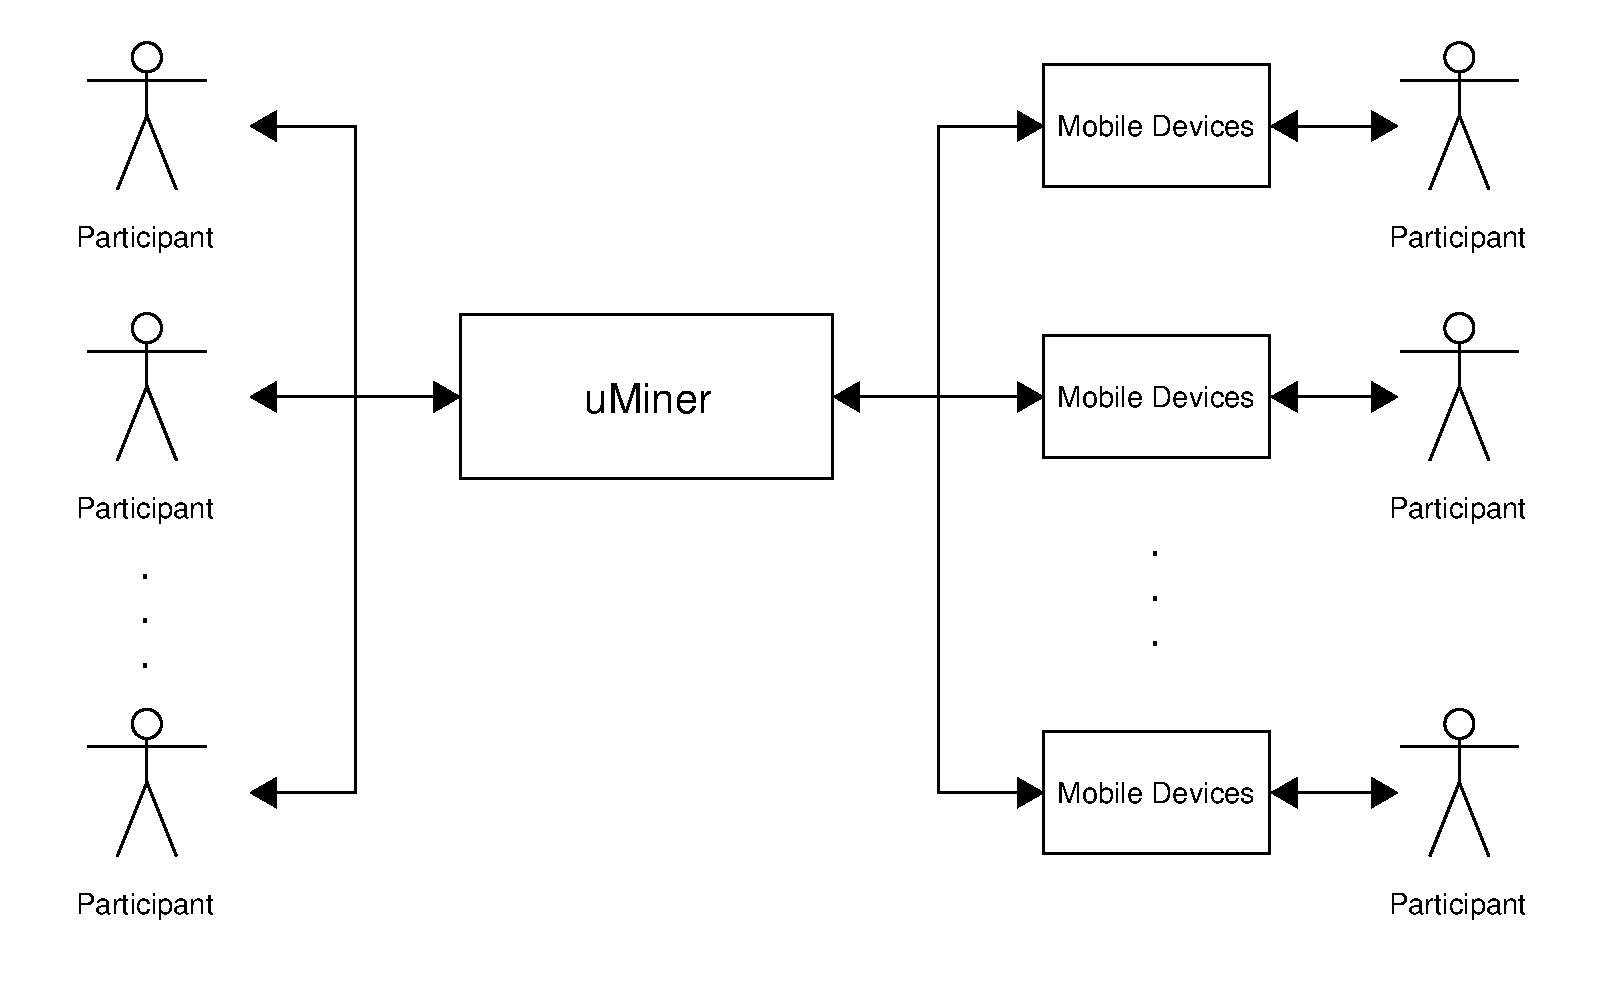
\includegraphics[width=\textwidth]{problem_analysis/vision/system_vision}
    \caption{The system vision.}
    \label{fig:system_vision}
\end{figure}
\FloatBarrier